\documentclass[twoside]{book}

% Packages required by doxygen
\usepackage{fixltx2e}
\usepackage{calc}
\usepackage{doxygen}
\usepackage[export]{adjustbox} % also loads graphicx
\usepackage{graphicx}
\usepackage[utf8]{inputenc}
\usepackage{makeidx}
\usepackage{multicol}
\usepackage{multirow}
\PassOptionsToPackage{warn}{textcomp}
\usepackage{textcomp}
\usepackage[nointegrals]{wasysym}
\usepackage[table]{xcolor}

% NLS support packages
\usepackage[spanish]{babel}
% Font selection
\usepackage[T1]{fontenc}
\usepackage[scaled=.90]{helvet}
\usepackage{courier}
\usepackage{amssymb}
\usepackage{sectsty}
\renewcommand{\familydefault}{\sfdefault}
\allsectionsfont{%
  \fontseries{bc}\selectfont%
  \color{darkgray}%
}
\renewcommand{\DoxyLabelFont}{%
  \fontseries{bc}\selectfont%
  \color{darkgray}%
}
\newcommand{\+}{\discretionary{\mbox{\scriptsize$\hookleftarrow$}}{}{}}

% Page & text layout
\usepackage{geometry}
\geometry{%
  a4paper,%
  top=2.5cm,%
  bottom=2.5cm,%
  left=2.5cm,%
  right=2.5cm%
}
\tolerance=750
\hfuzz=15pt
\hbadness=750
\setlength{\emergencystretch}{15pt}
\setlength{\parindent}{0cm}
\setlength{\parskip}{3ex plus 2ex minus 2ex}
\makeatletter
\renewcommand{\paragraph}{%
  \@startsection{paragraph}{4}{0ex}{-1.0ex}{1.0ex}{%
    \normalfont\normalsize\bfseries\SS@parafont%
  }%
}
\renewcommand{\subparagraph}{%
  \@startsection{subparagraph}{5}{0ex}{-1.0ex}{1.0ex}{%
    \normalfont\normalsize\bfseries\SS@subparafont%
  }%
}
\makeatother

% Headers & footers
\usepackage{fancyhdr}
\pagestyle{fancyplain}
\fancyhead[LE]{\fancyplain{}{\bfseries\thepage}}
\fancyhead[CE]{\fancyplain{}{}}
\fancyhead[RE]{\fancyplain{}{\bfseries\leftmark}}
\fancyhead[LO]{\fancyplain{}{\bfseries\rightmark}}
\fancyhead[CO]{\fancyplain{}{}}
\fancyhead[RO]{\fancyplain{}{\bfseries\thepage}}
\fancyfoot[LE]{\fancyplain{}{}}
\fancyfoot[CE]{\fancyplain{}{}}
\fancyfoot[RE]{\fancyplain{}{\bfseries\scriptsize Generado por Doxygen }}
\fancyfoot[LO]{\fancyplain{}{\bfseries\scriptsize Generado por Doxygen }}
\fancyfoot[CO]{\fancyplain{}{}}
\fancyfoot[RO]{\fancyplain{}{}}
\renewcommand{\footrulewidth}{0.4pt}
\renewcommand{\chaptermark}[1]{%
  \markboth{#1}{}%
}
\renewcommand{\sectionmark}[1]{%
  \markright{\thesection\ #1}%
}

% Indices & bibliography
\usepackage{natbib}
\usepackage[titles]{tocloft}
\setcounter{tocdepth}{3}
\setcounter{secnumdepth}{5}
\makeindex

% Hyperlinks (required, but should be loaded last)
\usepackage{ifpdf}
\ifpdf
  \usepackage[pdftex,pagebackref=true]{hyperref}
\else
  \usepackage[ps2pdf,pagebackref=true]{hyperref}
\fi
\hypersetup{%
  colorlinks=true,%
  linkcolor=blue,%
  citecolor=blue,%
  unicode%
}

% Custom commands
\newcommand{\clearemptydoublepage}{%
  \newpage{\pagestyle{empty}\cleardoublepage}%
}

\usepackage{caption}
\captionsetup{labelsep=space,justification=centering,font={bf},singlelinecheck=off,skip=4pt,position=top}

%===== C O N T E N T S =====

\begin{document}

% Titlepage & ToC
\hypersetup{pageanchor=false,
             bookmarksnumbered=true,
             pdfencoding=unicode
            }
\pagenumbering{alph}
\begin{titlepage}
\vspace*{7cm}
\begin{center}%
{\Large Arboles A\+VL \\[1ex]\large 1.\+0 }\\
\vspace*{1cm}
{\large Generado por Doxygen 1.8.13}\\
\end{center}
\end{titlepage}
\clearemptydoublepage
\pagenumbering{roman}
\tableofcontents
\clearemptydoublepage
\pagenumbering{arabic}
\hypersetup{pageanchor=true}

%--- Begin generated contents ---
\chapter{Equipo 3 -\/ Integrantes}
\label{index}\hypertarget{index}{}\begin{center}  \tabulinesep=1mm
\begin{longtabu} spread 0pt [c]{*{2}{|X[-1]}|}
\hline
\begin{center}\end{center} &\begin{center}\end{center}  \\\cline{1-2}
\PBS\centering {\itshape {\bfseries Facultad de Ciencias de la Computación}}&\PBS\centering {\itshape {\bfseries Benemérita Universidad Autónoma de Puebla}} \\\cline{1-2}
\multicolumn{2}{|p{(\linewidth-\tabcolsep*2-\arrayrulewidth*1)*2/2}|}{\PBS\centering {\bfseries Profesora} María del Carmen Santiago Díaz }\\\cline{1-2}
\multicolumn{2}{|p{(\linewidth-\tabcolsep*2-\arrayrulewidth*1)*2/2}|}{\PBS\centering Estructuras de Datos }\\\cline{1-2}
\multicolumn{2}{|p{(\linewidth-\tabcolsep*2-\arrayrulewidth*1)*2/2}|}{\PBS\centering {\itshape {\bfseries Manual técnico de T\+D\+As y Árboles A\+VL}} }\\\cline{1-2}
\end{longtabu}
~\newline
 \tabulinesep=1mm
\begin{longtabu} spread 0pt [c]{*{2}{|X[-1]}|}
\hline
\rowcolor{\tableheadbgcolor}\multicolumn{2}{|p{(\linewidth-\tabcolsep*2-\arrayrulewidth*1)*2/2}|}{\cellcolor{\tableheadbgcolor}\textbf{ Integrantes del equipo 3 }}\\\cline{1-2}
\endfirsthead
\hline
\endfoot
\hline
\rowcolor{\tableheadbgcolor}\multicolumn{2}{|p{(\linewidth-\tabcolsep*2-\arrayrulewidth*1)*2/2}|}{\cellcolor{\tableheadbgcolor}\textbf{ Integrantes del equipo 3 }}\\\cline{1-2}
\endhead
Batres Pedroza Alejandro&201836943 \\\cline{1-2}
García González Jorge&201847512 \\\cline{1-2}
Méndez Méndez Sebastián&201836190 \\\cline{1-2}
Segura Cuanalo Ricardo Alejandro&201848777 \\\cline{1-2}
\end{longtabu}
~\newline
 \subsection*{Introducción}\end{center} 

\begin{center} Este manual técnico fue realizado con el propósito de brindar una mejor comprensión para cualquiera que busque utilizar nuestros T\+D\+As, ya que esto podría ayudar al usuario a emplear nuestros algoritmos para diferentes tareas. Esto se pretende lograr, utilizando descripciones concisas para los métodos empleados, los parámetros de estos y las variables que contiene cada clase utilizada en el código.   \end{center} 

\begin{center}Ejecutables\+: \href{https://github.com/fcc-2018/arboles-avl/raw/master/ejecutables/arbolAVL.exe}{\tt Windows} -- \href{https://github.com/fcc-2018/arboles-avl/raw/master/ejecutables/arbolAVL}{\tt Linux}\end{center} 

\begin{center}  \end{center}  
\chapter{Indice jerárquico}
\section{Jerarquía de la clase}
Esta lista de herencias esta ordenada aproximadamente por orden alfabético\+:\begin{DoxyCompactList}
\item Grafo\begin{DoxyCompactList}
\item \contentsline{section}{Arbol}{\pageref{classArbol}}{}
\end{DoxyCompactList}
\end{DoxyCompactList}

\chapter{Índice de clases}
\section{Lista de clases}
Lista de las clases, estructuras, uniones e interfaces con una breve descripción\+:\begin{DoxyCompactList}
\item\contentsline{section}{\hyperlink{classArbol}{Arbol} \\*Implementación de un árbol binario con listas de adyacencia. ~\newline
 }{\pageref{classArbol}}{}
\item\contentsline{section}{\hyperlink{classArbolAVL}{Arbol\+A\+VL} \\*Implementación de un arbol binario que por cada inserción se corrobore el balance del mismo y se pueda auto-\/balancear }{\pageref{classArbolAVL}}{}
\item\contentsline{section}{\hyperlink{classArista}{Arista} \\*Clase que lleva el control del vertice de \textquotesingle{}origen\textquotesingle{} y de \textquotesingle{}destino\textquotesingle{} y el peso del camino entre estos }{\pageref{classArista}}{}
\item\contentsline{section}{\hyperlink{classcola}{cola$<$ T\+I\+P\+O $>$} \\*Clase que contiene las operaciones de una cola, haciendo uso de templates }{\pageref{classcola}}{}
\item\contentsline{section}{\hyperlink{classEtiqueta}{Etiqueta} \\*Clase de apoyo para conservar el Vértice Origen y su Peso }{\pageref{classEtiqueta}}{}
\item\contentsline{section}{\hyperlink{classGrafo}{Grafo} \\*Clase que contiene todos los procesos que se pueden realizar en el \hyperlink{classGrafo}{Grafo} }{\pageref{classGrafo}}{}
\item\contentsline{section}{\hyperlink{classLista_1_1iterator}{Lista$<$ tipo $>$\+::iterator} }{\pageref{classLista_1_1iterator}}{}
\item\contentsline{section}{\hyperlink{classLista}{Lista$<$ tipo $>$} }{\pageref{classLista}}{}
\item\contentsline{section}{\hyperlink{classMenu}{Menu} \\*Muestra un menu de opciones automaticamente y ejecuta el codigo que se le indica mediante funciones lambda en cada opcion }{\pageref{classMenu}}{}
\item\contentsline{section}{\hyperlink{classLista_1_1Nodo}{Lista$<$ tipo $>$\+::\+Nodo} }{\pageref{classLista_1_1Nodo}}{}
\item\contentsline{section}{\hyperlink{classnodo}{nodo$<$ T\+I\+P\+O $>$} \\*Clase que maneja los atributos escenciales de un nodo, haciendo uso de templates }{\pageref{classnodo}}{}
\item\contentsline{section}{\hyperlink{classnodos}{nodos$<$ T\+I\+P\+O $>$} }{\pageref{classnodos}}{}
\item\contentsline{section}{\hyperlink{classOpcion}{Opcion} \\*Representa a una opcion en el menu del programa }{\pageref{classOpcion}}{}
\item\contentsline{section}{\hyperlink{classpila}{pila$<$ T\+I\+P\+O $>$} }{\pageref{classpila}}{}
\item\contentsline{section}{\hyperlink{classVertice}{Vertice} \\*Clase encargada de llenar los datos en los Nodos insertados al \hyperlink{classGrafo}{Grafo} }{\pageref{classVertice}}{}
\end{DoxyCompactList}

\chapter{Indice de archivos}
\section{Lista de archivos}
Lista de todos los archivos documentados y con descripciones breves\+:\begin{DoxyCompactList}
\item\contentsline{section}{\hyperlink{arbol_8h}{arbol.\+h} }{\pageref{arbol_8h}}{}
\end{DoxyCompactList}

\chapter{Documentación de las clases}
\hypertarget{classArbol}{}\section{Referencia de la Clase Arbol}
\label{classArbol}\index{Arbol@{Arbol}}


Implementación de un arbol binario basada en un grafo con listas de adyacencia.  




{\ttfamily \#include $<$arbol.\+h$>$}



Diagrama de herencias de Arbol
% FIG 0


Diagrama de colaboración para Arbol\+:
% FIG 1
\subsection*{Métodos públicos}
\begin{DoxyCompactItemize}
\item 
\mbox{\Hypertarget{classArbol_a4f5d3e25a0e1a40cb09cefa39378b7be}\label{classArbol_a4f5d3e25a0e1a40cb09cefa39378b7be}} 
\hyperlink{classArbol_a4f5d3e25a0e1a40cb09cefa39378b7be}{Arbol} ()
\begin{DoxyCompactList}\small\item\em Constructor de la clase, se asume que la raíz del árbol es el primer vértice en la lista de adyacencia. \end{DoxyCompactList}\item 
int \hyperlink{classArbol_af332559b5f9d894ecc6a707bb1550ae2}{insertar} (int dato)
\begin{DoxyCompactList}\small\item\em Inserta un dato en el árbol. \end{DoxyCompactList}\item 
void \hyperlink{classArbol_a61749974f55056420f4e5a76eb664809}{mostrar} (ostream \&out)
\begin{DoxyCompactList}\small\item\em Muestra el árbol de manera horizontal. \end{DoxyCompactList}\item 
\mbox{\Hypertarget{classArbol_a5bd356760f63521e8578a83613aa4792}\label{classArbol_a5bd356760f63521e8578a83613aa4792}} 
void \hyperlink{classArbol_a5bd356760f63521e8578a83613aa4792}{recorrer} ()
\begin{DoxyCompactList}\small\item\em Muestra el árbol verticalmente. \end{DoxyCompactList}\item 
void \hyperlink{classArbol_a0ae46c572d300cd4a5f27b7d00a1a14e}{recorrer} (Vertice $\ast$raiz, int cont)
\begin{DoxyCompactList}\small\item\em Metodo recursivo auxiliar para \hyperlink{classArbol_a5bd356760f63521e8578a83613aa4792}{recorrer()} \end{DoxyCompactList}\item 
Lista$<$ Vertice $\ast$ $>$ $\ast$ \hyperlink{classArbol_a0ffdc60ce8f2267366681cc94cf6beea}{preorden} ()
\begin{DoxyCompactList}\small\item\em Recorre el árbol en preorden y los inserta en una lista. \end{DoxyCompactList}\item 
Lista$<$ Vertice $\ast$ $>$ $\ast$ \hyperlink{classArbol_a80a0c3cf2d7f3e92a5c8e5504947dab5}{inorden} ()
\begin{DoxyCompactList}\small\item\em Recorre el árbol en inorden y los inserta en una lista. \end{DoxyCompactList}\item 
\mbox{\Hypertarget{classArbol_a126e7d801dbe214ac39f183c26e9135d}\label{classArbol_a126e7d801dbe214ac39f183c26e9135d}} 
Lista$<$ Vertice $\ast$ $>$ $\ast$ \hyperlink{classArbol_a126e7d801dbe214ac39f183c26e9135d}{postorden} ()
\begin{DoxyCompactList}\small\item\em Recorre el árbol en inorden. \end{DoxyCompactList}\item 
int \hyperlink{classArbol_a9051a6b4120b42ff8d046f41ab73dbaa}{peso} ()
\begin{DoxyCompactList}\small\item\em Calcula el número de nodos en el árbol. \end{DoxyCompactList}\item 
int \hyperlink{classArbol_a99e608849650b891c34852a81f93d4ab}{grado} ()
\begin{DoxyCompactList}\small\item\em Calcula el grado del árbol, máximo número de hijos en cada nodo. \end{DoxyCompactList}\item 
Vertice $\ast$ \hyperlink{classArbol_abcb8c26e9021a1418de71ad6014351cf}{padre} (int hijo)
\begin{DoxyCompactList}\small\item\em Obtiene el padre de un nodo. \end{DoxyCompactList}\item 
Vertice $\ast$ \hyperlink{classArbol_a53527e7a8999ceda0b8a0fa25a3f357c}{padre} (string hijo)
\begin{DoxyCompactList}\small\item\em Obtiene el padre de un nodo. \end{DoxyCompactList}\item 
Vertice $\ast$ \hyperlink{classArbol_a3395234bc7b7a91d2880e10367039284}{padre} (Vertice $\ast$hijo)
\begin{DoxyCompactList}\small\item\em Obtiene el padre de un nodo. \end{DoxyCompactList}\item 
Lista$<$ Vertice $\ast$ $>$ $\ast$ \hyperlink{classArbol_ac2bfb4e9bab05342fb7d627fe3916183}{hijos} (int \hyperlink{classArbol_abcb8c26e9021a1418de71ad6014351cf}{padre})
\begin{DoxyCompactList}\small\item\em Obtiene los hijos de un vértice. \end{DoxyCompactList}\item 
Lista$<$ Vertice $\ast$ $>$ $\ast$ \hyperlink{classArbol_ac799e737e25e07d285d2bb29ba950b5c}{hijos} (string \hyperlink{classArbol_abcb8c26e9021a1418de71ad6014351cf}{padre})
\begin{DoxyCompactList}\small\item\em Obtiene los hijos de un vértice. \end{DoxyCompactList}\item 
Lista$<$ Vertice $\ast$ $>$ $\ast$ \hyperlink{classArbol_a54203315682d5c39015ae7d871223b66}{hojas} ()
\begin{DoxyCompactList}\small\item\em Obtiene las hojas del árbol. \end{DoxyCompactList}\item 
int \hyperlink{classArbol_aba59969b2a10294fb79e583a8e9471c5}{cont\+\_\+hojas} (Vertice $\ast$raiz)
\begin{DoxyCompactList}\small\item\em Calcula el número de hojas en el árbol. \end{DoxyCompactList}\item 
Vertice $\ast$ \hyperlink{classArbol_a59ae16f1a68c5e5afd08be20dcbf5717}{hermano} (int buscar)
\begin{DoxyCompactList}\small\item\em Obtiene el hermano de un vértice. \end{DoxyCompactList}\item 
bool \hyperlink{classArbol_a14ccdbb79a82bf19a24449acaea6c413}{es\+\_\+lleno} ()
\begin{DoxyCompactList}\small\item\em Verifica si el árbol cumple las condiciones de un árbol lleno, es decir cada nodo debe tener 0 o 2 hijos. \end{DoxyCompactList}\item 
bool \hyperlink{classArbol_a9e472df85f3bb1aa5c90f8157ad6ff22}{es\+\_\+completo\+\_\+o\+\_\+perfecto} ()
\begin{DoxyCompactList}\small\item\em Verifica si el árbol cumple las condiciones de un árbol perfecto/lleno ( árbol lleno con todas sus hojas en el mismo nivel ) \end{DoxyCompactList}\item 
int \hyperlink{classArbol_a98151655f0dab81b40d34f87fbbd90cd}{altura} (int dato)
\begin{DoxyCompactList}\small\item\em Calcula la altura de un nodo. \end{DoxyCompactList}\item 
int \hyperlink{classArbol_a7a79cb43ca30b5120f1a8ebe3afbe22c}{altura} (string nombre)
\begin{DoxyCompactList}\small\item\em Calcula la altura de un nodo. \end{DoxyCompactList}\item 
int \hyperlink{classArbol_a9f8928b4c72e2d484ef75cf3633c22ce}{altura} (Vertice $\ast$nodo)
\begin{DoxyCompactList}\small\item\em Calcula la altura de un nodo. \end{DoxyCompactList}\item 
int \hyperlink{classArbol_accd2dd2f8012067c1a2d77fd14c64546}{nivel} (int dato)
\begin{DoxyCompactList}\small\item\em Calcula el nivel donde se encuentra un nodo. \end{DoxyCompactList}\item 
int \hyperlink{classArbol_a3a8a414e8e3f45bf90c481649928a86d}{nivel} (string nombre)
\begin{DoxyCompactList}\small\item\em Calcula el nivel donde se encuentra un nodo. \end{DoxyCompactList}\item 
Lista$<$ Vertice $\ast$ $>$ $\ast$ \hyperlink{classArbol_ac7ff5e2f436a1e83e24cbdd0b2cc827b}{antecesores} (int dato)
\begin{DoxyCompactList}\small\item\em Obtiene los antecesores de un nodo. \end{DoxyCompactList}\item 
Lista$<$ Vertice $\ast$ $>$ $\ast$ \hyperlink{classArbol_aa975d5d9cf5fcfc392a8200bd0078d1c}{antecesores} (string nombre)
\begin{DoxyCompactList}\small\item\em Obtiene los antecesores de un nodo. \end{DoxyCompactList}\item 
Lista$<$ Vertice $\ast$ $>$ $\ast$ \hyperlink{classArbol_acae8e9dfd17ae18e250d9029172e1c9e}{descendientes} (int dato)
\begin{DoxyCompactList}\small\item\em Obtiene los descendientes de un nodo. \end{DoxyCompactList}\item 
Lista$<$ Vertice $\ast$ $>$ $\ast$ \hyperlink{classArbol_a790b07f284b14bd179499eb4a991ad86}{descendientes} (string nombre)
\begin{DoxyCompactList}\small\item\em Obtiene los descendientes de un nodo. \end{DoxyCompactList}\item 
Lista$<$ Vertice $\ast$ $>$ $\ast$ \hyperlink{classArbol_accfa606c5f5e67b6ab18c4490075cf39}{camino\+\_\+entre} (int o, int d)
\begin{DoxyCompactList}\small\item\em Obtiene el un camino entre dos vértices en el árbol. \end{DoxyCompactList}\item 
Lista$<$ Vertice $\ast$ $>$ $\ast$ \hyperlink{classArbol_aef0f680828ac573af495b98d2eb09c12}{camino\+\_\+entre} (string origen, string destino)
\begin{DoxyCompactList}\small\item\em Obtiene el un camino entre dos vértices en el árbol. \end{DoxyCompactList}\end{DoxyCompactItemize}
\subsection*{Métodos protegidos}
\begin{DoxyCompactItemize}
\item 
void \hyperlink{classArbol_a707f748c57d51f6b63fe1a605476e49d}{\+\_\+\+\_\+preorden\+\_\+\+\_\+} (Vertice $\ast$raiz, Lista$<$ Vertice $\ast$$>$ $\ast$lista)
\begin{DoxyCompactList}\small\item\em Recorre un árbol en preorden (Visitar, Izquierda, Derecha) recursivamente, método auxiliar de \hyperlink{classArbol_a0ffdc60ce8f2267366681cc94cf6beea}{preorden()} \end{DoxyCompactList}\item 
void \hyperlink{classArbol_ae3dc89f7db1fb9b54bcc2489eb1d9542}{\+\_\+\+\_\+inorden\+\_\+\+\_\+} (Vertice $\ast$raiz, Lista$<$ Vertice $\ast$$>$ $\ast$lista)
\begin{DoxyCompactList}\small\item\em Recorre un árbol en inorden (Izquierda, Visitar, Derecha) recursivamente, método auxiliar de \hyperlink{classArbol_a80a0c3cf2d7f3e92a5c8e5504947dab5}{inorden()} \end{DoxyCompactList}\item 
void \hyperlink{classArbol_aea4cc9147a79d74956413a233df1dbe0}{\+\_\+\+\_\+postorden\+\_\+\+\_\+} (Vertice $\ast$raiz, Lista$<$ Vertice $\ast$$>$ $\ast$lista)
\begin{DoxyCompactList}\small\item\em Recorre un árbol en postorden (Izquierda, Derecha, Visitar) recursivamente, método auxiliar de \hyperlink{classArbol_a126e7d801dbe214ac39f183c26e9135d}{postorden()} \end{DoxyCompactList}\item 
void \hyperlink{classArbol_a1e00baa76d846e9e586e7d179ec51907}{\+\_\+\+\_\+camino\+\_\+\+\_\+} (Vertice $\ast$origen, Vertice $\ast$destino, Lista$<$ Vertice $\ast$$>$ $\ast$$\ast$camino)
\begin{DoxyCompactList}\small\item\em Obtiene el camino entre 2 vértices en el árbol, método auxiliar de \hyperlink{classArbol_accfa606c5f5e67b6ab18c4490075cf39}{camino\+\_\+entre()} \end{DoxyCompactList}\item 
int \hyperlink{classArbol_ad3077ad7b0c57ed7c98baa7fcd8aab47}{\+\_\+\+\_\+grado\+\_\+\+\_\+} (Vertice $\ast$raiz)
\begin{DoxyCompactList}\small\item\em Obtiene el grado de un árbol de manera recursiva. \end{DoxyCompactList}\item 
int \hyperlink{classArbol_ab34b0a58f349a2f8153911ad4821a9b9}{\+\_\+\+\_\+altura\+\_\+\+\_\+} (Vertice $\ast$v)
\begin{DoxyCompactList}\small\item\em Obtiene la altura de un árbol recursivamente. \end{DoxyCompactList}\item 
int \hyperlink{classArbol_a479d9841f100bf75b87fb2155b66d591}{\+\_\+\+\_\+nivel\+\_\+\+\_\+} (Vertice $\ast$raiz, Vertice $\ast$vert, int lvl)
\begin{DoxyCompactList}\small\item\em Obtiene el nivel de un nodo en el árbol. \end{DoxyCompactList}\item 
void \hyperlink{classArbol_aad97c679cb368931b2c6894b3dbcb60f}{\+\_\+\+\_\+hojas\+\_\+\+\_\+} (Vertice $\ast$raiz, Lista$<$ Vertice $\ast$$>$ $\ast$lista)
\begin{DoxyCompactList}\small\item\em Obtiene las hojas de un árbol. \end{DoxyCompactList}\item 
void \hyperlink{classArbol_a1e3da012e6667062976bca9f78efef7e}{\+\_\+\+\_\+hijos\+\_\+\+\_\+} (Vertice $\ast$raiz, Vertice $\ast$\hyperlink{classArbol_abcb8c26e9021a1418de71ad6014351cf}{padre}, Lista$<$ Vertice $\ast$$>$ $\ast$lista)
\begin{DoxyCompactList}\small\item\em Obtiene los hijos de un nodo dado. \end{DoxyCompactList}\item 
void \hyperlink{classArbol_a495a7502a29e01ce7fa168daca651b1f}{\+\_\+\+\_\+padre\+\_\+\+\_\+} (Vertice $\ast$raiz, Vertice $\ast$hijo, Vertice $\ast$$\ast$\hyperlink{classArbol_abcb8c26e9021a1418de71ad6014351cf}{padre})
\begin{DoxyCompactList}\small\item\em Obtiene el padre de un nodo dado. \end{DoxyCompactList}\item 
void \hyperlink{classArbol_aeb7dff584795382d8e8a1a4694d0ac4e}{ordenar\+\_\+lista\+\_\+de\+\_\+adyacentes} (Lista$<$ Vertice $\ast$$>$ $\ast$lista)
\begin{DoxyCompactList}\small\item\em Ordena una lista de vértices en orden ascendente. \end{DoxyCompactList}\item 
Vertice $\ast$$\ast$ \hyperlink{classArbol_a18066699977ab8095398d026ef2a13ac}{obtener\+\_\+hijos} (Vertice $\ast$\hyperlink{classArbol_abcb8c26e9021a1418de71ad6014351cf}{padre})
\begin{DoxyCompactList}\small\item\em Obtiene los hijos de un vértice en orden ascendente. \end{DoxyCompactList}\item 
bool \hyperlink{classArbol_aba4b09fef18152beb43e04fee7394f34}{todos\+\_\+cumplen\+\_\+con} (bool($\ast$funcion\+\_\+callback)(Vertice $\ast$))
\begin{DoxyCompactList}\small\item\em Verifica que todos los vértices en el árbol cumplen una condición dada por una función de callback. \end{DoxyCompactList}\item 
bool \hyperlink{classArbol_a60b71d79b81a3a1083709ec264332975}{\+\_\+\+\_\+todos\+\_\+cumplen\+\_\+con\+\_\+\+\_\+} (bool($\ast$funcion\+\_\+callback)(Vertice $\ast$), Vertice $\ast$vert)
\begin{DoxyCompactList}\small\item\em Método auxiliar para \hyperlink{classArbol_aba4b09fef18152beb43e04fee7394f34}{todos\+\_\+cumplen\+\_\+con()} verifica la condición en cada nodo del árbol recursivamente. \end{DoxyCompactList}\end{DoxyCompactItemize}


\subsection{Descripción detallada}
Implementación de un arbol binario basada en un grafo con listas de adyacencia. 

Definición en la línea 30 del archivo arbol.\+h.



\subsection{Documentación de las funciones miembro}
\mbox{\Hypertarget{classArbol_ab34b0a58f349a2f8153911ad4821a9b9}\label{classArbol_ab34b0a58f349a2f8153911ad4821a9b9}} 
\index{Arbol@{Arbol}!\+\_\+\+\_\+altura\+\_\+\+\_\+@{\+\_\+\+\_\+altura\+\_\+\+\_\+}}
\index{\+\_\+\+\_\+altura\+\_\+\+\_\+@{\+\_\+\+\_\+altura\+\_\+\+\_\+}!Arbol@{Arbol}}
\subsubsection{\texorpdfstring{\+\_\+\+\_\+altura\+\_\+\+\_\+()}{\_\_altura\_\_()}}
{\footnotesize\ttfamily int Arbol\+::\+\_\+\+\_\+altura\+\_\+\+\_\+ (\begin{DoxyParamCaption}\item[{Vertice $\ast$}]{v }\end{DoxyParamCaption})\hspace{0.3cm}{\ttfamily [protected]}}



Obtiene la altura de un árbol recursivamente. 


\begin{DoxyParams}{Parámetros}
{\em v} & puntero a vértice raíz del árbol \\
\hline
\end{DoxyParams}
\begin{DoxyReturn}{Devuelve}
altura del árbol 0 si es hoja 
\end{DoxyReturn}


Definición en la línea 937 del archivo arbol.\+h.

\mbox{\Hypertarget{classArbol_a1e00baa76d846e9e586e7d179ec51907}\label{classArbol_a1e00baa76d846e9e586e7d179ec51907}} 
\index{Arbol@{Arbol}!\+\_\+\+\_\+camino\+\_\+\+\_\+@{\+\_\+\+\_\+camino\+\_\+\+\_\+}}
\index{\+\_\+\+\_\+camino\+\_\+\+\_\+@{\+\_\+\+\_\+camino\+\_\+\+\_\+}!Arbol@{Arbol}}
\subsubsection{\texorpdfstring{\+\_\+\+\_\+camino\+\_\+\+\_\+()}{\_\_camino\_\_()}}
{\footnotesize\ttfamily void Arbol\+::\+\_\+\+\_\+camino\+\_\+\+\_\+ (\begin{DoxyParamCaption}\item[{Vertice $\ast$}]{origen,  }\item[{Vertice $\ast$}]{destino,  }\item[{Lista$<$ Vertice $\ast$$>$ $\ast$$\ast$}]{camino }\end{DoxyParamCaption})\hspace{0.3cm}{\ttfamily [protected]}}



Obtiene el camino entre 2 vértices en el árbol, método auxiliar de \hyperlink{classArbol_accfa606c5f5e67b6ab18c4490075cf39}{camino\+\_\+entre()} 


\begin{DoxyParams}{Parámetros}
{\em origen} & puntero a vértice de inicial del camino \\
\hline
{\em destino} & puntero a vértice final del camino \\
\hline
{\em camino} & doble puntero a lista de vértices donde se guardarán los nodos en orden \\
\hline
\end{DoxyParams}


Definición en la línea 877 del archivo arbol.\+h.

\mbox{\Hypertarget{classArbol_ad3077ad7b0c57ed7c98baa7fcd8aab47}\label{classArbol_ad3077ad7b0c57ed7c98baa7fcd8aab47}} 
\index{Arbol@{Arbol}!\+\_\+\+\_\+grado\+\_\+\+\_\+@{\+\_\+\+\_\+grado\+\_\+\+\_\+}}
\index{\+\_\+\+\_\+grado\+\_\+\+\_\+@{\+\_\+\+\_\+grado\+\_\+\+\_\+}!Arbol@{Arbol}}
\subsubsection{\texorpdfstring{\+\_\+\+\_\+grado\+\_\+\+\_\+()}{\_\_grado\_\_()}}
{\footnotesize\ttfamily int Arbol\+::\+\_\+\+\_\+grado\+\_\+\+\_\+ (\begin{DoxyParamCaption}\item[{Vertice $\ast$}]{raiz }\end{DoxyParamCaption})\hspace{0.3cm}{\ttfamily [protected]}}



Obtiene el grado de un árbol de manera recursiva. 


\begin{DoxyParams}{Parámetros}
{\em raiz} & puntero a vértice raíz del árbol \\
\hline
\end{DoxyParams}
\begin{DoxyReturn}{Devuelve}
int número más grande de hijos en nodos del árbol 
\end{DoxyReturn}


Definición en la línea 593 del archivo arbol.\+h.

\mbox{\Hypertarget{classArbol_a1e3da012e6667062976bca9f78efef7e}\label{classArbol_a1e3da012e6667062976bca9f78efef7e}} 
\index{Arbol@{Arbol}!\+\_\+\+\_\+hijos\+\_\+\+\_\+@{\+\_\+\+\_\+hijos\+\_\+\+\_\+}}
\index{\+\_\+\+\_\+hijos\+\_\+\+\_\+@{\+\_\+\+\_\+hijos\+\_\+\+\_\+}!Arbol@{Arbol}}
\subsubsection{\texorpdfstring{\+\_\+\+\_\+hijos\+\_\+\+\_\+()}{\_\_hijos\_\_()}}
{\footnotesize\ttfamily void Arbol\+::\+\_\+\+\_\+hijos\+\_\+\+\_\+ (\begin{DoxyParamCaption}\item[{Vertice $\ast$}]{raiz,  }\item[{Vertice $\ast$}]{padre,  }\item[{Lista$<$ Vertice $\ast$$>$ $\ast$}]{lista }\end{DoxyParamCaption})\hspace{0.3cm}{\ttfamily [protected]}}



Obtiene los hijos de un nodo dado. 


\begin{DoxyParams}{Parámetros}
{\em raiz} & del árbol donde se buscará el nodo \\
\hline
{\em padre} & puntero al nodo que se quieren obtener los nodos hijos \\
\hline
{\em lista} & puntero a lista de vértices donde se guardarán los hijos del nodo \\
\hline
\end{DoxyParams}


Definición en la línea 388 del archivo arbol.\+h.

\mbox{\Hypertarget{classArbol_aad97c679cb368931b2c6894b3dbcb60f}\label{classArbol_aad97c679cb368931b2c6894b3dbcb60f}} 
\index{Arbol@{Arbol}!\+\_\+\+\_\+hojas\+\_\+\+\_\+@{\+\_\+\+\_\+hojas\+\_\+\+\_\+}}
\index{\+\_\+\+\_\+hojas\+\_\+\+\_\+@{\+\_\+\+\_\+hojas\+\_\+\+\_\+}!Arbol@{Arbol}}
\subsubsection{\texorpdfstring{\+\_\+\+\_\+hojas\+\_\+\+\_\+()}{\_\_hojas\_\_()}}
{\footnotesize\ttfamily void Arbol\+::\+\_\+\+\_\+hojas\+\_\+\+\_\+ (\begin{DoxyParamCaption}\item[{Vertice $\ast$}]{raiz,  }\item[{Lista$<$ Vertice $\ast$$>$ $\ast$}]{lista }\end{DoxyParamCaption})\hspace{0.3cm}{\ttfamily [protected]}}



Obtiene las hojas de un árbol. 


\begin{DoxyParams}{Parámetros}
{\em raiz} & puntero a raíz del subárbol \\
\hline
{\em lista} & puntero a lista de vértices donde se guardarán los vértices hojas \\
\hline
\end{DoxyParams}


Definición en la línea 469 del archivo arbol.\+h.

\mbox{\Hypertarget{classArbol_ae3dc89f7db1fb9b54bcc2489eb1d9542}\label{classArbol_ae3dc89f7db1fb9b54bcc2489eb1d9542}} 
\index{Arbol@{Arbol}!\+\_\+\+\_\+inorden\+\_\+\+\_\+@{\+\_\+\+\_\+inorden\+\_\+\+\_\+}}
\index{\+\_\+\+\_\+inorden\+\_\+\+\_\+@{\+\_\+\+\_\+inorden\+\_\+\+\_\+}!Arbol@{Arbol}}
\subsubsection{\texorpdfstring{\+\_\+\+\_\+inorden\+\_\+\+\_\+()}{\_\_inorden\_\_()}}
{\footnotesize\ttfamily void Arbol\+::\+\_\+\+\_\+inorden\+\_\+\+\_\+ (\begin{DoxyParamCaption}\item[{Vertice $\ast$}]{raiz,  }\item[{Lista$<$ Vertice $\ast$$>$ $\ast$}]{lista }\end{DoxyParamCaption})\hspace{0.3cm}{\ttfamily [protected]}}



Recorre un árbol en inorden (Izquierda, Visitar, Derecha) recursivamente, método auxiliar de \hyperlink{classArbol_a80a0c3cf2d7f3e92a5c8e5504947dab5}{inorden()} 


\begin{DoxyParams}{Parámetros}
{\em raiz} & puntero a la raíz del árbol a recorrer \\
\hline
{\em lista} & puntero a lista de vertices (donde se guardarán los vértices visitados en orden) \\
\hline
\end{DoxyParams}


Definición en la línea 527 del archivo arbol.\+h.

\mbox{\Hypertarget{classArbol_a479d9841f100bf75b87fb2155b66d591}\label{classArbol_a479d9841f100bf75b87fb2155b66d591}} 
\index{Arbol@{Arbol}!\+\_\+\+\_\+nivel\+\_\+\+\_\+@{\+\_\+\+\_\+nivel\+\_\+\+\_\+}}
\index{\+\_\+\+\_\+nivel\+\_\+\+\_\+@{\+\_\+\+\_\+nivel\+\_\+\+\_\+}!Arbol@{Arbol}}
\subsubsection{\texorpdfstring{\+\_\+\+\_\+nivel\+\_\+\+\_\+()}{\_\_nivel\_\_()}}
{\footnotesize\ttfamily int Arbol\+::\+\_\+\+\_\+nivel\+\_\+\+\_\+ (\begin{DoxyParamCaption}\item[{Vertice $\ast$}]{raiz,  }\item[{Vertice $\ast$}]{vert,  }\item[{int}]{lvl }\end{DoxyParamCaption})\hspace{0.3cm}{\ttfamily [protected]}}



Obtiene el nivel de un nodo en el árbol. 


\begin{DoxyParams}{Parámetros}
{\em raiz} & puntero a raíz del árbol donde se buscará el nodo \\
\hline
{\em vert} & puntero a vértice que se encontrará su nivel \\
\hline
{\em lvl} & nivel actual en el subárbol \\
\hline
\end{DoxyParams}
\begin{DoxyReturn}{Devuelve}
nivel del nodo apuntado por vert 
\end{DoxyReturn}


Definición en la línea 961 del archivo arbol.\+h.

\mbox{\Hypertarget{classArbol_a495a7502a29e01ce7fa168daca651b1f}\label{classArbol_a495a7502a29e01ce7fa168daca651b1f}} 
\index{Arbol@{Arbol}!\+\_\+\+\_\+padre\+\_\+\+\_\+@{\+\_\+\+\_\+padre\+\_\+\+\_\+}}
\index{\+\_\+\+\_\+padre\+\_\+\+\_\+@{\+\_\+\+\_\+padre\+\_\+\+\_\+}!Arbol@{Arbol}}
\subsubsection{\texorpdfstring{\+\_\+\+\_\+padre\+\_\+\+\_\+()}{\_\_padre\_\_()}}
{\footnotesize\ttfamily void Arbol\+::\+\_\+\+\_\+padre\+\_\+\+\_\+ (\begin{DoxyParamCaption}\item[{Vertice $\ast$}]{raiz,  }\item[{Vertice $\ast$}]{hijo,  }\item[{Vertice $\ast$$\ast$}]{padre }\end{DoxyParamCaption})\hspace{0.3cm}{\ttfamily [protected]}}



Obtiene el padre de un nodo dado. 


\begin{DoxyParams}{Parámetros}
{\em raiz} & puntero a la raíz del subárbol \\
\hline
{\em padre} & doble puntero a un vértice donde se pondrá la direccion de memoria del padre \\
\hline
\end{DoxyParams}


Definición en la línea 427 del archivo arbol.\+h.

\mbox{\Hypertarget{classArbol_aea4cc9147a79d74956413a233df1dbe0}\label{classArbol_aea4cc9147a79d74956413a233df1dbe0}} 
\index{Arbol@{Arbol}!\+\_\+\+\_\+postorden\+\_\+\+\_\+@{\+\_\+\+\_\+postorden\+\_\+\+\_\+}}
\index{\+\_\+\+\_\+postorden\+\_\+\+\_\+@{\+\_\+\+\_\+postorden\+\_\+\+\_\+}!Arbol@{Arbol}}
\subsubsection{\texorpdfstring{\+\_\+\+\_\+postorden\+\_\+\+\_\+()}{\_\_postorden\_\_()}}
{\footnotesize\ttfamily void Arbol\+::\+\_\+\+\_\+postorden\+\_\+\+\_\+ (\begin{DoxyParamCaption}\item[{Vertice $\ast$}]{raiz,  }\item[{Lista$<$ Vertice $\ast$$>$ $\ast$}]{lista }\end{DoxyParamCaption})\hspace{0.3cm}{\ttfamily [protected]}}



Recorre un árbol en postorden (Izquierda, Derecha, Visitar) recursivamente, método auxiliar de \hyperlink{classArbol_a126e7d801dbe214ac39f183c26e9135d}{postorden()} 


\begin{DoxyParams}{Parámetros}
{\em raiz} & puntero a vértice raíz del árbol \\
\hline
{\em lista} & puntero a lista de vértices (donde se guardarán los vértices visitados en orden) \\
\hline
\end{DoxyParams}


Definición en la línea 575 del archivo arbol.\+h.

\mbox{\Hypertarget{classArbol_a707f748c57d51f6b63fe1a605476e49d}\label{classArbol_a707f748c57d51f6b63fe1a605476e49d}} 
\index{Arbol@{Arbol}!\+\_\+\+\_\+preorden\+\_\+\+\_\+@{\+\_\+\+\_\+preorden\+\_\+\+\_\+}}
\index{\+\_\+\+\_\+preorden\+\_\+\+\_\+@{\+\_\+\+\_\+preorden\+\_\+\+\_\+}!Arbol@{Arbol}}
\subsubsection{\texorpdfstring{\+\_\+\+\_\+preorden\+\_\+\+\_\+()}{\_\_preorden\_\_()}}
{\footnotesize\ttfamily void Arbol\+::\+\_\+\+\_\+preorden\+\_\+\+\_\+ (\begin{DoxyParamCaption}\item[{Vertice $\ast$}]{raiz,  }\item[{Lista$<$ Vertice $\ast$$>$ $\ast$}]{lista }\end{DoxyParamCaption})\hspace{0.3cm}{\ttfamily [protected]}}



Recorre un árbol en preorden (Visitar, Izquierda, Derecha) recursivamente, método auxiliar de \hyperlink{classArbol_a0ffdc60ce8f2267366681cc94cf6beea}{preorden()} 


\begin{DoxyParams}{Parámetros}
{\em raiz} & puntero a la raíz del árbol a recorrer \\
\hline
{\em lista} & puntero a lista de vértices (donde se guardarán los vértices visitados en orden) \\
\hline
\end{DoxyParams}


Definición en la línea 504 del archivo arbol.\+h.

\mbox{\Hypertarget{classArbol_a60b71d79b81a3a1083709ec264332975}\label{classArbol_a60b71d79b81a3a1083709ec264332975}} 
\index{Arbol@{Arbol}!\+\_\+\+\_\+todos\+\_\+cumplen\+\_\+con\+\_\+\+\_\+@{\+\_\+\+\_\+todos\+\_\+cumplen\+\_\+con\+\_\+\+\_\+}}
\index{\+\_\+\+\_\+todos\+\_\+cumplen\+\_\+con\+\_\+\+\_\+@{\+\_\+\+\_\+todos\+\_\+cumplen\+\_\+con\+\_\+\+\_\+}!Arbol@{Arbol}}
\subsubsection{\texorpdfstring{\+\_\+\+\_\+todos\+\_\+cumplen\+\_\+con\+\_\+\+\_\+()}{\_\_todos\_cumplen\_con\_\_()}}
{\footnotesize\ttfamily bool Arbol\+::\+\_\+\+\_\+todos\+\_\+cumplen\+\_\+con\+\_\+\+\_\+ (\begin{DoxyParamCaption}\item[{bool($\ast$)(Vertice $\ast$)}]{funcion\+\_\+callback,  }\item[{Vertice $\ast$}]{vert }\end{DoxyParamCaption})\hspace{0.3cm}{\ttfamily [protected]}}



Método auxiliar para \hyperlink{classArbol_aba4b09fef18152beb43e04fee7394f34}{todos\+\_\+cumplen\+\_\+con()} verifica la condición en cada nodo del árbol recursivamente. 


\begin{DoxyParams}{Parámetros}
{\em funcion\+\_\+callback} & función que verifica una condición en un solo vértice \\
\hline
{\em vert} & puntero a vértice raíz del subárbol \\
\hline
\end{DoxyParams}
\begin{DoxyReturn}{Devuelve}
true si los nodos en el subárbol cumplen la condicion, false en caso contrario. 
\end{DoxyReturn}


Definición en la línea 548 del archivo arbol.\+h.

\mbox{\Hypertarget{classArbol_a98151655f0dab81b40d34f87fbbd90cd}\label{classArbol_a98151655f0dab81b40d34f87fbbd90cd}} 
\index{Arbol@{Arbol}!altura@{altura}}
\index{altura@{altura}!Arbol@{Arbol}}
\subsubsection{\texorpdfstring{altura()}{altura()}\hspace{0.1cm}{\footnotesize\ttfamily [1/3]}}
{\footnotesize\ttfamily int Arbol\+::altura (\begin{DoxyParamCaption}\item[{int}]{dato }\end{DoxyParamCaption})}



Calcula la altura de un nodo. 


\begin{DoxyParams}{Parámetros}
{\em dato} & valor numérico del nodo \\
\hline
\end{DoxyParams}
\begin{DoxyReturn}{Devuelve}
int altura 
\end{DoxyReturn}


Definición en la línea 909 del archivo arbol.\+h.

\mbox{\Hypertarget{classArbol_a7a79cb43ca30b5120f1a8ebe3afbe22c}\label{classArbol_a7a79cb43ca30b5120f1a8ebe3afbe22c}} 
\index{Arbol@{Arbol}!altura@{altura}}
\index{altura@{altura}!Arbol@{Arbol}}
\subsubsection{\texorpdfstring{altura()}{altura()}\hspace{0.1cm}{\footnotesize\ttfamily [2/3]}}
{\footnotesize\ttfamily int Arbol\+::altura (\begin{DoxyParamCaption}\item[{string}]{nombre }\end{DoxyParamCaption})}



Calcula la altura de un nodo. 


\begin{DoxyParams}{Parámetros}
{\em nombre} & nombre del vértice \\
\hline
\end{DoxyParams}
\begin{DoxyReturn}{Devuelve}
int altura 
\end{DoxyReturn}


Definición en la línea 915 del archivo arbol.\+h.

\mbox{\Hypertarget{classArbol_a9f8928b4c72e2d484ef75cf3633c22ce}\label{classArbol_a9f8928b4c72e2d484ef75cf3633c22ce}} 
\index{Arbol@{Arbol}!altura@{altura}}
\index{altura@{altura}!Arbol@{Arbol}}
\subsubsection{\texorpdfstring{altura()}{altura()}\hspace{0.1cm}{\footnotesize\ttfamily [3/3]}}
{\footnotesize\ttfamily int Arbol\+::altura (\begin{DoxyParamCaption}\item[{Vertice $\ast$}]{nodo }\end{DoxyParamCaption})}



Calcula la altura de un nodo. 


\begin{DoxyParams}{Parámetros}
{\em nodo} & puntero al nodo \\
\hline
\end{DoxyParams}
\begin{DoxyReturn}{Devuelve}
int altura 
\end{DoxyReturn}


Definición en la línea 927 del archivo arbol.\+h.

\mbox{\Hypertarget{classArbol_ac7ff5e2f436a1e83e24cbdd0b2cc827b}\label{classArbol_ac7ff5e2f436a1e83e24cbdd0b2cc827b}} 
\index{Arbol@{Arbol}!antecesores@{antecesores}}
\index{antecesores@{antecesores}!Arbol@{Arbol}}
\subsubsection{\texorpdfstring{antecesores()}{antecesores()}\hspace{0.1cm}{\footnotesize\ttfamily [1/2]}}
{\footnotesize\ttfamily Lista$<$ Vertice $\ast$ $>$ $\ast$ Arbol\+::antecesores (\begin{DoxyParamCaption}\item[{int}]{dato }\end{DoxyParamCaption})}



Obtiene los antecesores de un nodo. 


\begin{DoxyParams}{Parámetros}
{\em dato} & valor numérico del nodo \\
\hline
\end{DoxyParams}
\begin{DoxyReturn}{Devuelve}
lista de punteros a vértices previos al nodo 
\end{DoxyReturn}


Definición en la línea 978 del archivo arbol.\+h.

\mbox{\Hypertarget{classArbol_aa975d5d9cf5fcfc392a8200bd0078d1c}\label{classArbol_aa975d5d9cf5fcfc392a8200bd0078d1c}} 
\index{Arbol@{Arbol}!antecesores@{antecesores}}
\index{antecesores@{antecesores}!Arbol@{Arbol}}
\subsubsection{\texorpdfstring{antecesores()}{antecesores()}\hspace{0.1cm}{\footnotesize\ttfamily [2/2]}}
{\footnotesize\ttfamily Lista$<$ Vertice $\ast$ $>$ $\ast$ Arbol\+::antecesores (\begin{DoxyParamCaption}\item[{string}]{nombre }\end{DoxyParamCaption})}



Obtiene los antecesores de un nodo. 


\begin{DoxyParams}{Parámetros}
{\em nombre} & nombre del nodo raíz \\
\hline
\end{DoxyParams}
\begin{DoxyReturn}{Devuelve}
lista de punteros a vértices antecesores al nodo 
\end{DoxyReturn}


Definición en la línea 982 del archivo arbol.\+h.

\mbox{\Hypertarget{classArbol_accfa606c5f5e67b6ab18c4490075cf39}\label{classArbol_accfa606c5f5e67b6ab18c4490075cf39}} 
\index{Arbol@{Arbol}!camino\+\_\+entre@{camino\+\_\+entre}}
\index{camino\+\_\+entre@{camino\+\_\+entre}!Arbol@{Arbol}}
\subsubsection{\texorpdfstring{camino\+\_\+entre()}{camino\_entre()}\hspace{0.1cm}{\footnotesize\ttfamily [1/2]}}
{\footnotesize\ttfamily Lista$<$ Vertice $\ast$ $>$ $\ast$ Arbol\+::camino\+\_\+entre (\begin{DoxyParamCaption}\item[{int}]{o,  }\item[{int}]{d }\end{DoxyParamCaption})}



Obtiene el un camino entre dos vértices en el árbol. 


\begin{DoxyParams}{Parámetros}
{\em o} & valor numérico del vértice origen \\
\hline
{\em d} & valor numérico del vértice destino \\
\hline
\end{DoxyParams}
\begin{DoxyReturn}{Devuelve}
lista de punteros a vértices en el camnino de o a d 
\end{DoxyReturn}


Definición en la línea 862 del archivo arbol.\+h.

\mbox{\Hypertarget{classArbol_aef0f680828ac573af495b98d2eb09c12}\label{classArbol_aef0f680828ac573af495b98d2eb09c12}} 
\index{Arbol@{Arbol}!camino\+\_\+entre@{camino\+\_\+entre}}
\index{camino\+\_\+entre@{camino\+\_\+entre}!Arbol@{Arbol}}
\subsubsection{\texorpdfstring{camino\+\_\+entre()}{camino\_entre()}\hspace{0.1cm}{\footnotesize\ttfamily [2/2]}}
{\footnotesize\ttfamily Lista$<$ Vertice $\ast$ $>$ $\ast$ Arbol\+::camino\+\_\+entre (\begin{DoxyParamCaption}\item[{string}]{origen,  }\item[{string}]{destino }\end{DoxyParamCaption})}



Obtiene el un camino entre dos vértices en el árbol. 


\begin{DoxyParams}{Parámetros}
{\em origen} & nombre del vértice origen \\
\hline
{\em destino} & nombre del vértice destino \\
\hline
\end{DoxyParams}
\begin{DoxyReturn}{Devuelve}
lista de punteros a vértices en el camnino de origen a destino 
\end{DoxyReturn}


Definición en la línea 866 del archivo arbol.\+h.

\mbox{\Hypertarget{classArbol_aba59969b2a10294fb79e583a8e9471c5}\label{classArbol_aba59969b2a10294fb79e583a8e9471c5}} 
\index{Arbol@{Arbol}!cont\+\_\+hojas@{cont\+\_\+hojas}}
\index{cont\+\_\+hojas@{cont\+\_\+hojas}!Arbol@{Arbol}}
\subsubsection{\texorpdfstring{cont\+\_\+hojas()}{cont\_hojas()}}
{\footnotesize\ttfamily int Arbol\+::cont\+\_\+hojas (\begin{DoxyParamCaption}\item[{Vertice $\ast$}]{raiz }\end{DoxyParamCaption})}



Calcula el número de hojas en el árbol. 


\begin{DoxyParams}{Parámetros}
{\em raiz} & puntero a vértice raíz del árbol \\
\hline
\end{DoxyParams}
\begin{DoxyReturn}{Devuelve}
lista de punteros a vértices hijos 
\end{DoxyReturn}


Definición en la línea 440 del archivo arbol.\+h.

\mbox{\Hypertarget{classArbol_acae8e9dfd17ae18e250d9029172e1c9e}\label{classArbol_acae8e9dfd17ae18e250d9029172e1c9e}} 
\index{Arbol@{Arbol}!descendientes@{descendientes}}
\index{descendientes@{descendientes}!Arbol@{Arbol}}
\subsubsection{\texorpdfstring{descendientes()}{descendientes()}\hspace{0.1cm}{\footnotesize\ttfamily [1/2]}}
{\footnotesize\ttfamily Lista$<$ Vertice $\ast$ $>$ $\ast$ Arbol\+::descendientes (\begin{DoxyParamCaption}\item[{int}]{dato }\end{DoxyParamCaption})}



Obtiene los descendientes de un nodo. 


\begin{DoxyParams}{Parámetros}
{\em dato} & valor numérico del nodo raíz \\
\hline
\end{DoxyParams}
\begin{DoxyReturn}{Devuelve}
lista de punteros a vértices descendientes al nodo 
\end{DoxyReturn}


Definición en la línea 993 del archivo arbol.\+h.

\mbox{\Hypertarget{classArbol_a790b07f284b14bd179499eb4a991ad86}\label{classArbol_a790b07f284b14bd179499eb4a991ad86}} 
\index{Arbol@{Arbol}!descendientes@{descendientes}}
\index{descendientes@{descendientes}!Arbol@{Arbol}}
\subsubsection{\texorpdfstring{descendientes()}{descendientes()}\hspace{0.1cm}{\footnotesize\ttfamily [2/2]}}
{\footnotesize\ttfamily Lista$<$ Vertice $\ast$ $>$ $\ast$ Arbol\+::descendientes (\begin{DoxyParamCaption}\item[{string}]{nombre }\end{DoxyParamCaption})}



Obtiene los descendientes de un nodo. 


\begin{DoxyParams}{Parámetros}
{\em nombre} & nombre del nodo raíz \\
\hline
\end{DoxyParams}
\begin{DoxyReturn}{Devuelve}
lista de punteros a vértices descendientes al nodo 
\end{DoxyReturn}


Definición en la línea 999 del archivo arbol.\+h.

\mbox{\Hypertarget{classArbol_a9e472df85f3bb1aa5c90f8157ad6ff22}\label{classArbol_a9e472df85f3bb1aa5c90f8157ad6ff22}} 
\index{Arbol@{Arbol}!es\+\_\+completo\+\_\+o\+\_\+perfecto@{es\+\_\+completo\+\_\+o\+\_\+perfecto}}
\index{es\+\_\+completo\+\_\+o\+\_\+perfecto@{es\+\_\+completo\+\_\+o\+\_\+perfecto}!Arbol@{Arbol}}
\subsubsection{\texorpdfstring{es\+\_\+completo\+\_\+o\+\_\+perfecto()}{es\_completo\_o\_perfecto()}}
{\footnotesize\ttfamily bool Arbol\+::es\+\_\+completo\+\_\+o\+\_\+perfecto (\begin{DoxyParamCaption}{ }\end{DoxyParamCaption})}



Verifica si el árbol cumple las condiciones de un árbol perfecto/lleno ( árbol lleno con todas sus hojas en el mismo nivel ) 

\begin{DoxyReturn}{Devuelve}
true si es perfecto, false en caso contrario 
\end{DoxyReturn}


Definición en la línea 845 del archivo arbol.\+h.

\mbox{\Hypertarget{classArbol_a14ccdbb79a82bf19a24449acaea6c413}\label{classArbol_a14ccdbb79a82bf19a24449acaea6c413}} 
\index{Arbol@{Arbol}!es\+\_\+lleno@{es\+\_\+lleno}}
\index{es\+\_\+lleno@{es\+\_\+lleno}!Arbol@{Arbol}}
\subsubsection{\texorpdfstring{es\+\_\+lleno()}{es\_lleno()}}
{\footnotesize\ttfamily bool Arbol\+::es\+\_\+lleno (\begin{DoxyParamCaption}{ }\end{DoxyParamCaption})}



Verifica si el árbol cumple las condiciones de un árbol lleno, es decir cada nodo debe tener 0 o 2 hijos. 

\begin{DoxyReturn}{Devuelve}
true si el árbol es lleno, false en caso contrario 
\end{DoxyReturn}


Definición en la línea 833 del archivo arbol.\+h.

\mbox{\Hypertarget{classArbol_a99e608849650b891c34852a81f93d4ab}\label{classArbol_a99e608849650b891c34852a81f93d4ab}} 
\index{Arbol@{Arbol}!grado@{grado}}
\index{grado@{grado}!Arbol@{Arbol}}
\subsubsection{\texorpdfstring{grado()}{grado()}}
{\footnotesize\ttfamily int Arbol\+::grado (\begin{DoxyParamCaption}{ }\end{DoxyParamCaption})}



Calcula el grado del árbol, máximo número de hijos en cada nodo. 

\begin{DoxyReturn}{Devuelve}
grado 
\end{DoxyReturn}


Definición en la línea 589 del archivo arbol.\+h.

\mbox{\Hypertarget{classArbol_a59ae16f1a68c5e5afd08be20dcbf5717}\label{classArbol_a59ae16f1a68c5e5afd08be20dcbf5717}} 
\index{Arbol@{Arbol}!hermano@{hermano}}
\index{hermano@{hermano}!Arbol@{Arbol}}
\subsubsection{\texorpdfstring{hermano()}{hermano()}}
{\footnotesize\ttfamily Vertice $\ast$ Arbol\+::hermano (\begin{DoxyParamCaption}\item[{int}]{buscar }\end{DoxyParamCaption})}



Obtiene el hermano de un vértice. 


\begin{DoxyParams}{Parámetros}
{\em buscar} & valor numérico del hermano del vértice buscar \\
\hline
\end{DoxyParams}
\begin{DoxyReturn}{Devuelve}
puntero a vértice hermano 
\end{DoxyReturn}


Definición en la línea 358 del archivo arbol.\+h.

\mbox{\Hypertarget{classArbol_ac2bfb4e9bab05342fb7d627fe3916183}\label{classArbol_ac2bfb4e9bab05342fb7d627fe3916183}} 
\index{Arbol@{Arbol}!hijos@{hijos}}
\index{hijos@{hijos}!Arbol@{Arbol}}
\subsubsection{\texorpdfstring{hijos()}{hijos()}\hspace{0.1cm}{\footnotesize\ttfamily [1/2]}}
{\footnotesize\ttfamily Lista$<$ Vertice $\ast$ $>$ $\ast$ Arbol\+::hijos (\begin{DoxyParamCaption}\item[{int}]{padre }\end{DoxyParamCaption})}



Obtiene los hijos de un vértice. 


\begin{DoxyParams}{Parámetros}
{\em padre} & valor numérico del vértice padre \\
\hline
\end{DoxyParams}
\begin{DoxyReturn}{Devuelve}
lista de punteros a vértices hijos 
\end{DoxyReturn}


Definición en la línea 376 del archivo arbol.\+h.

\mbox{\Hypertarget{classArbol_ac799e737e25e07d285d2bb29ba950b5c}\label{classArbol_ac799e737e25e07d285d2bb29ba950b5c}} 
\index{Arbol@{Arbol}!hijos@{hijos}}
\index{hijos@{hijos}!Arbol@{Arbol}}
\subsubsection{\texorpdfstring{hijos()}{hijos()}\hspace{0.1cm}{\footnotesize\ttfamily [2/2]}}
{\footnotesize\ttfamily Lista$<$ Vertice $\ast$ $>$ $\ast$ Arbol\+::hijos (\begin{DoxyParamCaption}\item[{string}]{padre }\end{DoxyParamCaption})}



Obtiene los hijos de un vértice. 


\begin{DoxyParams}{Parámetros}
{\em padre} & nombre del vértice padre \\
\hline
\end{DoxyParams}
\begin{DoxyReturn}{Devuelve}
lista de punteros a vértices hijos 
\end{DoxyReturn}


Definición en la línea 380 del archivo arbol.\+h.

\mbox{\Hypertarget{classArbol_a54203315682d5c39015ae7d871223b66}\label{classArbol_a54203315682d5c39015ae7d871223b66}} 
\index{Arbol@{Arbol}!hojas@{hojas}}
\index{hojas@{hojas}!Arbol@{Arbol}}
\subsubsection{\texorpdfstring{hojas()}{hojas()}}
{\footnotesize\ttfamily Lista$<$ Vertice $\ast$ $>$ $\ast$ Arbol\+::hojas (\begin{DoxyParamCaption}{ }\end{DoxyParamCaption})}



Obtiene las hojas del árbol. 

\begin{DoxyReturn}{Devuelve}
lista de punteros a vértices hojas 
\end{DoxyReturn}


Definición en la línea 461 del archivo arbol.\+h.

\mbox{\Hypertarget{classArbol_a80a0c3cf2d7f3e92a5c8e5504947dab5}\label{classArbol_a80a0c3cf2d7f3e92a5c8e5504947dab5}} 
\index{Arbol@{Arbol}!inorden@{inorden}}
\index{inorden@{inorden}!Arbol@{Arbol}}
\subsubsection{\texorpdfstring{inorden()}{inorden()}}
{\footnotesize\ttfamily Lista$<$ Vertice $\ast$ $>$ $\ast$ Arbol\+::inorden (\begin{DoxyParamCaption}{ }\end{DoxyParamCaption})}



Recorre el árbol en inorden y los inserta en una lista. 

\begin{DoxyReturn}{Devuelve}
Lista de punteros a vértices del arbol en inorden 
\end{DoxyReturn}


Definición en la línea 517 del archivo arbol.\+h.

\mbox{\Hypertarget{classArbol_af332559b5f9d894ecc6a707bb1550ae2}\label{classArbol_af332559b5f9d894ecc6a707bb1550ae2}} 
\index{Arbol@{Arbol}!insertar@{insertar}}
\index{insertar@{insertar}!Arbol@{Arbol}}
\subsubsection{\texorpdfstring{insertar()}{insertar()}}
{\footnotesize\ttfamily int Arbol\+::insertar (\begin{DoxyParamCaption}\item[{int}]{dato }\end{DoxyParamCaption})}



Inserta un dato en el árbol. 


\begin{DoxyParams}{Parámetros}
{\em dato} & número a insertar \\
\hline
\end{DoxyParams}
\begin{DoxyReturn}{Devuelve}
Nivel en el que fué insertado el nodo 
\end{DoxyReturn}


Definición en la línea 752 del archivo arbol.\+h.

\mbox{\Hypertarget{classArbol_a61749974f55056420f4e5a76eb664809}\label{classArbol_a61749974f55056420f4e5a76eb664809}} 
\index{Arbol@{Arbol}!mostrar@{mostrar}}
\index{mostrar@{mostrar}!Arbol@{Arbol}}
\subsubsection{\texorpdfstring{mostrar()}{mostrar()}}
{\footnotesize\ttfamily void Arbol\+::mostrar (\begin{DoxyParamCaption}\item[{ostream \&}]{out }\end{DoxyParamCaption})}



Muestra el árbol de manera horizontal. 


\begin{DoxyParams}{Parámetros}
{\em out} & Referencia a un flujo de salida \\
\hline
\end{DoxyParams}


Definición en la línea 689 del archivo arbol.\+h.

\mbox{\Hypertarget{classArbol_accd2dd2f8012067c1a2d77fd14c64546}\label{classArbol_accd2dd2f8012067c1a2d77fd14c64546}} 
\index{Arbol@{Arbol}!nivel@{nivel}}
\index{nivel@{nivel}!Arbol@{Arbol}}
\subsubsection{\texorpdfstring{nivel()}{nivel()}\hspace{0.1cm}{\footnotesize\ttfamily [1/2]}}
{\footnotesize\ttfamily int Arbol\+::nivel (\begin{DoxyParamCaption}\item[{int}]{dato }\end{DoxyParamCaption})}



Calcula el nivel donde se encuentra un nodo. 


\begin{DoxyParams}{Parámetros}
{\em dato} & valor numérico del nodo \\
\hline
\end{DoxyParams}
\begin{DoxyReturn}{Devuelve}
int nivel 
\end{DoxyReturn}


Definición en la línea 949 del archivo arbol.\+h.

\mbox{\Hypertarget{classArbol_a3a8a414e8e3f45bf90c481649928a86d}\label{classArbol_a3a8a414e8e3f45bf90c481649928a86d}} 
\index{Arbol@{Arbol}!nivel@{nivel}}
\index{nivel@{nivel}!Arbol@{Arbol}}
\subsubsection{\texorpdfstring{nivel()}{nivel()}\hspace{0.1cm}{\footnotesize\ttfamily [2/2]}}
{\footnotesize\ttfamily int Arbol\+::nivel (\begin{DoxyParamCaption}\item[{string}]{nombre }\end{DoxyParamCaption})}



Calcula el nivel donde se encuentra un nodo. 


\begin{DoxyParams}{Parámetros}
{\em nombre} & nombre del nodo \\
\hline
\end{DoxyParams}
\begin{DoxyReturn}{Devuelve}
int nivel 
\end{DoxyReturn}


Definición en la línea 953 del archivo arbol.\+h.

\mbox{\Hypertarget{classArbol_a18066699977ab8095398d026ef2a13ac}\label{classArbol_a18066699977ab8095398d026ef2a13ac}} 
\index{Arbol@{Arbol}!obtener\+\_\+hijos@{obtener\+\_\+hijos}}
\index{obtener\+\_\+hijos@{obtener\+\_\+hijos}!Arbol@{Arbol}}
\subsubsection{\texorpdfstring{obtener\+\_\+hijos()}{obtener\_hijos()}}
{\footnotesize\ttfamily Vertice $\ast$$\ast$ Arbol\+::obtener\+\_\+hijos (\begin{DoxyParamCaption}\item[{Vertice $\ast$}]{padre }\end{DoxyParamCaption})\hspace{0.3cm}{\ttfamily [protected]}}



Obtiene los hijos de un vértice en orden ascendente. 


\begin{DoxyParams}{Parámetros}
{\em padre} & vértice padre \\
\hline
\end{DoxyParams}
\begin{DoxyReturn}{Devuelve}
Arreglo de vértices de longitud 2, hijos\mbox{[}0\mbox{]} hijo izquierdo de padre, hijos\mbox{[}1\mbox{]} hijo derecho de padre 
\end{DoxyReturn}


Definición en la línea 612 del archivo arbol.\+h.

\mbox{\Hypertarget{classArbol_aeb7dff584795382d8e8a1a4694d0ac4e}\label{classArbol_aeb7dff584795382d8e8a1a4694d0ac4e}} 
\index{Arbol@{Arbol}!ordenar\+\_\+lista\+\_\+de\+\_\+adyacentes@{ordenar\+\_\+lista\+\_\+de\+\_\+adyacentes}}
\index{ordenar\+\_\+lista\+\_\+de\+\_\+adyacentes@{ordenar\+\_\+lista\+\_\+de\+\_\+adyacentes}!Arbol@{Arbol}}
\subsubsection{\texorpdfstring{ordenar\+\_\+lista\+\_\+de\+\_\+adyacentes()}{ordenar\_lista\_de\_adyacentes()}}
{\footnotesize\ttfamily void Arbol\+::ordenar\+\_\+lista\+\_\+de\+\_\+adyacentes (\begin{DoxyParamCaption}\item[{Lista$<$ Vertice $\ast$$>$ $\ast$}]{lista }\end{DoxyParamCaption})\hspace{0.3cm}{\ttfamily [protected]}}



Ordena una lista de vértices en orden ascendente. 


\begin{DoxyParams}{Parámetros}
{\em lista} & puntero a lista de vertices a ordenar \\
\hline
\end{DoxyParams}


Definición en la línea 657 del archivo arbol.\+h.

\mbox{\Hypertarget{classArbol_abcb8c26e9021a1418de71ad6014351cf}\label{classArbol_abcb8c26e9021a1418de71ad6014351cf}} 
\index{Arbol@{Arbol}!padre@{padre}}
\index{padre@{padre}!Arbol@{Arbol}}
\subsubsection{\texorpdfstring{padre()}{padre()}\hspace{0.1cm}{\footnotesize\ttfamily [1/3]}}
{\footnotesize\ttfamily Vertice $\ast$ Arbol\+::padre (\begin{DoxyParamCaption}\item[{int}]{hijo }\end{DoxyParamCaption})}



Obtiene el padre de un nodo. 


\begin{DoxyParams}{Parámetros}
{\em hijo} & valor numérico del vértice hijo \\
\hline
\end{DoxyParams}
\begin{DoxyReturn}{Devuelve}
puntero a vértice padre o N\+U\+LL si el hijo no existe 
\end{DoxyReturn}


Definición en la línea 403 del archivo arbol.\+h.

\mbox{\Hypertarget{classArbol_a53527e7a8999ceda0b8a0fa25a3f357c}\label{classArbol_a53527e7a8999ceda0b8a0fa25a3f357c}} 
\index{Arbol@{Arbol}!padre@{padre}}
\index{padre@{padre}!Arbol@{Arbol}}
\subsubsection{\texorpdfstring{padre()}{padre()}\hspace{0.1cm}{\footnotesize\ttfamily [2/3]}}
{\footnotesize\ttfamily Vertice $\ast$ Arbol\+::padre (\begin{DoxyParamCaption}\item[{string}]{hijo }\end{DoxyParamCaption})}



Obtiene el padre de un nodo. 


\begin{DoxyParams}{Parámetros}
{\em hijo} & nombre del vértice hijo \\
\hline
\end{DoxyParams}
\begin{DoxyReturn}{Devuelve}
puntero a vértice padre o N\+U\+LL si el hijo no existe 
\end{DoxyReturn}


Definición en la línea 408 del archivo arbol.\+h.

\mbox{\Hypertarget{classArbol_a3395234bc7b7a91d2880e10367039284}\label{classArbol_a3395234bc7b7a91d2880e10367039284}} 
\index{Arbol@{Arbol}!padre@{padre}}
\index{padre@{padre}!Arbol@{Arbol}}
\subsubsection{\texorpdfstring{padre()}{padre()}\hspace{0.1cm}{\footnotesize\ttfamily [3/3]}}
{\footnotesize\ttfamily Vertice $\ast$ Arbol\+::padre (\begin{DoxyParamCaption}\item[{Vertice $\ast$}]{hijo }\end{DoxyParamCaption})}



Obtiene el padre de un nodo. 


\begin{DoxyParams}{Parámetros}
{\em hijo} & puntero a vértice hijo \\
\hline
\end{DoxyParams}
\begin{DoxyReturn}{Devuelve}
puntero a vértice padre 
\end{DoxyReturn}


Definición en la línea 418 del archivo arbol.\+h.

\mbox{\Hypertarget{classArbol_a9051a6b4120b42ff8d046f41ab73dbaa}\label{classArbol_a9051a6b4120b42ff8d046f41ab73dbaa}} 
\index{Arbol@{Arbol}!peso@{peso}}
\index{peso@{peso}!Arbol@{Arbol}}
\subsubsection{\texorpdfstring{peso()}{peso()}}
{\footnotesize\ttfamily int Arbol\+::peso (\begin{DoxyParamCaption}{ }\end{DoxyParamCaption})}



Calcula el número de nodos en el árbol. 

\begin{DoxyReturn}{Devuelve}
numero de nodos 
\end{DoxyReturn}


Definición en la línea 584 del archivo arbol.\+h.

\mbox{\Hypertarget{classArbol_a0ffdc60ce8f2267366681cc94cf6beea}\label{classArbol_a0ffdc60ce8f2267366681cc94cf6beea}} 
\index{Arbol@{Arbol}!preorden@{preorden}}
\index{preorden@{preorden}!Arbol@{Arbol}}
\subsubsection{\texorpdfstring{preorden()}{preorden()}}
{\footnotesize\ttfamily Lista$<$ Vertice $\ast$ $>$ $\ast$ Arbol\+::preorden (\begin{DoxyParamCaption}{ }\end{DoxyParamCaption})}



Recorre el árbol en preorden y los inserta en una lista. 

\begin{DoxyReturn}{Devuelve}
Lista de punteros a vértices del árbol en preorden 
\end{DoxyReturn}


Definición en la línea 492 del archivo arbol.\+h.

\mbox{\Hypertarget{classArbol_a0ae46c572d300cd4a5f27b7d00a1a14e}\label{classArbol_a0ae46c572d300cd4a5f27b7d00a1a14e}} 
\index{Arbol@{Arbol}!recorrer@{recorrer}}
\index{recorrer@{recorrer}!Arbol@{Arbol}}
\subsubsection{\texorpdfstring{recorrer()}{recorrer()}}
{\footnotesize\ttfamily void Arbol\+::recorrer (\begin{DoxyParamCaption}\item[{Vertice $\ast$}]{raiz,  }\item[{int}]{cont }\end{DoxyParamCaption})}



Metodo recursivo auxiliar para \hyperlink{classArbol_a5bd356760f63521e8578a83613aa4792}{recorrer()} 


\begin{DoxyParams}{Parámetros}
{\em raiz} & puntero a la raíz del arbol a mostrar \\
\hline
{\em cont} & contador del nivel del nodo actual (cont = 0) \\
\hline
\end{DoxyParams}


Definición en la línea 801 del archivo arbol.\+h.

\mbox{\Hypertarget{classArbol_aba4b09fef18152beb43e04fee7394f34}\label{classArbol_aba4b09fef18152beb43e04fee7394f34}} 
\index{Arbol@{Arbol}!todos\+\_\+cumplen\+\_\+con@{todos\+\_\+cumplen\+\_\+con}}
\index{todos\+\_\+cumplen\+\_\+con@{todos\+\_\+cumplen\+\_\+con}!Arbol@{Arbol}}
\subsubsection{\texorpdfstring{todos\+\_\+cumplen\+\_\+con()}{todos\_cumplen\_con()}}
{\footnotesize\ttfamily bool Arbol\+::todos\+\_\+cumplen\+\_\+con (\begin{DoxyParamCaption}\item[{bool($\ast$)(Vertice $\ast$)}]{funcion\+\_\+callback }\end{DoxyParamCaption})\hspace{0.3cm}{\ttfamily [protected]}}



Verifica que todos los vértices en el árbol cumplen una condición dada por una función de callback. 


\begin{DoxyParams}{Parámetros}
{\em funcion\+\_\+callback} & función que verifica una condición en un solo vértice \\
\hline
\end{DoxyParams}
\begin{DoxyReturn}{Devuelve}
true si todos los vértices pasan la prueba false si no. 
\end{DoxyReturn}


Definición en la línea 544 del archivo arbol.\+h.



La documentación para esta clase fue generada a partir del siguiente fichero\+:\begin{DoxyCompactItemize}
\item 
\hyperlink{arbol_8h}{arbol.\+h}\end{DoxyCompactItemize}

\chapter{Documentación de archivos}
\hypertarget{arbol_8h}{}\section{Referencia del Archivo arbol.\+h}
\label{arbol_8h}\index{arbol.\+h@{arbol.\+h}}


Definción de clase \hyperlink{classArbol}{Arbol} e implementación de sus métodos.  


{\ttfamily \#include $<$iostream$>$}\newline
{\ttfamily \#include $<$cmath$>$}\newline
{\ttfamily \#include $<$string$>$}\newline
{\ttfamily \#include \char`\"{}grafo.\+h\char`\"{}}\newline
{\ttfamily \#include \char`\"{}pila.\+h\char`\"{}}\newline
Dependencia gráfica adjunta para arbol.\+h\+:\nopagebreak
\begin{figure}[H]
\begin{center}
\leavevmode
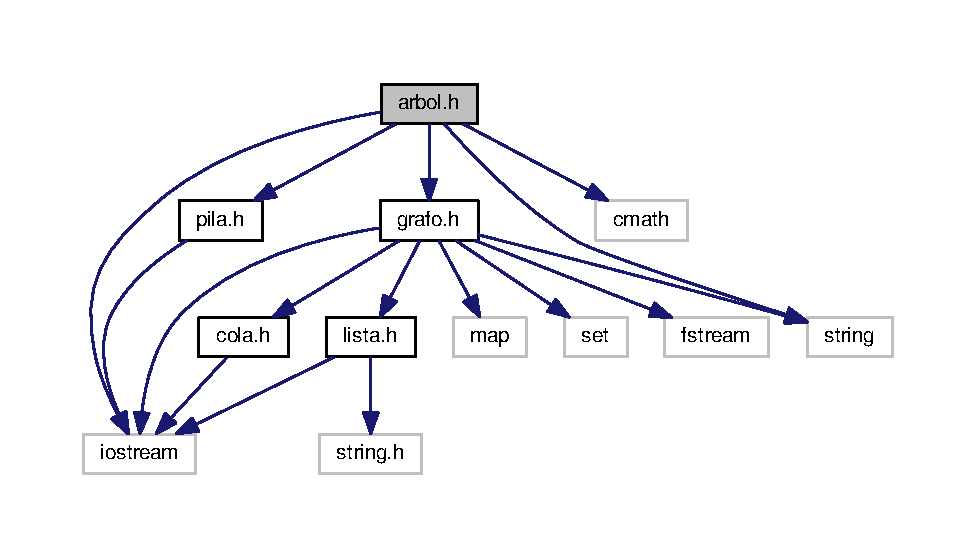
\includegraphics[width=350pt]{arbol_8h__incl}
\end{center}
\end{figure}
Gráfico de los archivos que directa o indirectamente incluyen a este archivo\+:\nopagebreak
\begin{figure}[H]
\begin{center}
\leavevmode
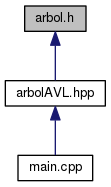
\includegraphics[width=155pt]{arbol_8h__dep__incl}
\end{center}
\end{figure}
\subsection*{Clases}
\begin{DoxyCompactItemize}
\item 
class \hyperlink{classArbol}{Arbol}
\begin{DoxyCompactList}\small\item\em Implementación de un árbol binario con listas de adyacencia. ~\newline
 \end{DoxyCompactList}\end{DoxyCompactItemize}
\subsection*{Funciones}
\begin{DoxyCompactItemize}
\item 
\mbox{\Hypertarget{arbol_8h_a01910d4b2446ba5d0e062ecb24a13b6d}\label{arbol_8h_a01910d4b2446ba5d0e062ecb24a13b6d}} 
bool {\bfseries dos\+\_\+o\+\_\+cero\+\_\+hijos} (\hyperlink{classVertice}{Vertice} $\ast$vert)
\end{DoxyCompactItemize}


\subsection{Descripción detallada}
Definción de clase \hyperlink{classArbol}{Arbol} e implementación de sus métodos. 


%--- End generated contents ---

% Index
\backmatter
\newpage
\phantomsection
\clearemptydoublepage
\addcontentsline{toc}{chapter}{Índice}
\printindex

\end{document}
